\chapter{操作系统的启动过程}
\label{cha:OSboot}

\section{基本输入输出系统(BIOS)}
\label{sec:BIOS}

BIOS的全称是Basic Input/Output System,意思就是基本输入输出系统。它是计
算机上第一个运行的软件。当然,它不可能自己加载自己,那么它就只能是由硬
件来加载了,而这个硬件就是CPU\cite{zg2016}。在计算机通电
瞬间,如图\ref{fig:img2-1}所示,寄存器\texttt{CS:IP}会被赋予一个初
值:\texttt{F000:FFF0}。之后,CPU将会执行下面这条指令:
\begin{codeblock}
\begin{nasmcode}
jmp f000:e05b
\end{nasmcode}
\end{codeblock}
\texttt{JMP},顾名思义就是要跳转到内存中的\texttt{F000:E05B}这个地址,
这里就是BIOS待机的地方。\texttt{JMP}到这之后,BIOS被唤醒,接管了CPU的使用权
。之后BIOS要做的事情就是:
\begin{itemize}
\item 准备好和基本输入输出相关的函数
\item 检查硬件
\item 将主引导扇区(MBR)的代码加载到内存中的\texttt{0x7C00}位置
\item 跳转到\texttt{0x7C00}
\end{itemize}

\begin{figure}[H]
  \centering
  \includegraphics[width=.9\linewidth]{图2-1}  
  \caption{Bochs屏幕截图}
  \label{fig:img2-1}
\end{figure}

\section{MBR的工作}
\label{sec:MBR}

MBR,全称是Master Boot Record,主引导扇区,共有512个字节,其结构如图\ref{fig:mbr}所
示。主要由三个部分组成,分别是:
\begin{itemize}
\item 主引导程序(Bootloader):占扇区前446个字节,在计算机开机,BIOS完成自检后,会将MBR加载
  到内存中,然后执行前446字节的引导程序。
\item 硬盘分区表(DPT):占扇区中间64个字节,主要用来定位各个分区,访问用户数据。
\item MBR结束标志\texttt{0xAA55}:占扇区最后2字节,也被称为魔数。每次执行引导程序时都会检查
  程序的结尾是否是\texttt{0xAA55},若不是的话则会认定这是一个无效的MBR引导扇区,将会中止引
  导。
\end{itemize}

\begin{figure}
  \centering
  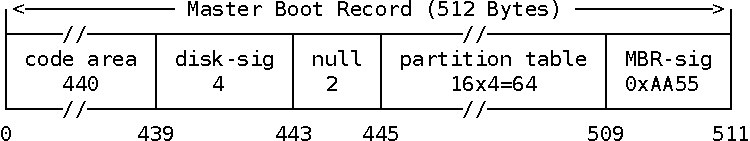
\includegraphics[width=.7\textwidth]{mbr}
  \caption{MBR的结构}
  \label{fig:mbr}
\end{figure}

BIOS在\texttt{0x7C00}处把CPU的控制权交由MBR之后,将会再次进入待机状
态,至此,BIOS的任务就完成了。\texttt{MBR.S}中的代码部分是由自己编写的,它可
以简单到只要如下三条汇编程序语句:%
\begin{itemize}
\item 告诉汇编器把MBR的起始地址编译为\texttt{0x7C00};
\begin{codeblock}
\begin{nasmcode}
 SECTION MBR vstart=0x7c00
\end{nasmcode}
\end{codeblock}
\item \verb'$'表示本行所在的地址,\verb'$-$$'意思是本行到本section的偏移量,MBR必须得填满
  512个字节,而最后两个是固定的\texttt{0x55}和\texttt{0xAA},所以剩下空着的部分用0来填充。
\begin{codeblock}
\begin{nasmcode}
 times 510-($-$$) db 0 
\end{nasmcode}
\end{codeblock}
\item MBR结束;
\begin{codeblock}
\begin{nasmcode}
 db 0x55,0xaa  
\end{nasmcode}
\end{codeblock}  
\end{itemize}

这样就拥有了一个很小的MBR,当然只是这样做的话,屏幕上可能会有很
多乱七八糟的信息,因为Bochs虚拟机的设计师默认是会显示一些Bochs
的版本号等等信息的,所以还是让Bochs的界面能够显示的清爽一些,调
用汇编寄存器\texttt{0x60}号功能号来实现清屏,再通过对字符串的
操作来实现在Bochs界面上打印出来一个\texttt{Hello, OS world!}
来表示MBR已经被成功加载了。代码如下:%

\begin{longlisting}
\begin{nasmcode}
    org 07c00h          ; 告诉编译器程序加载到7c00处
    mov ax, cs          
    mov ds, ax          
    mov es, ax          
    mov ah, 0x6         ; 利用0x60号功能清屏
    mov al, 0x0         ; AL = 上卷的行数(0表示全部)
    mov bx, 0x700
    mov cx, 0x0
    mov dx, 0x184f
    int 10h
    call DispStr        ; 调用显示字符串例程
    jmp $               ; 无限循环
DispStr:
    mov ax, BootMessage
    mov bp, ax          ; ES:BP = 串地址
    mov cx, 16          ; CX = 串长度
    mov ax, 01301h      ; AH = 13,  AL = 01h
    mov bx, 000ch       ; 页号为0(BH = 0) 黑底红字(BL = 0Ch,高亮)
    mov dl, 0
    int 10h             ; 10h 号中断
    ret
BootMessage:        db  "Hello, OS world!"

times   510-($-$$)  db  0   ; 填充剩下的空间,使生成的二进制代码恰好为512字节
dw  0xaa55                  ; 结束标志
\end{nasmcode}
\end{longlisting}

如图\ref{fig:img2-2}所示,一个最小的操作系统就完成了。

\begin{figure}[H]
  \centering
  \includegraphics[width=.7\linewidth]{图2-2}
  \caption{Hello, OS World!}
  \label{fig:img2-2}
\end{figure}

至此,MBR已经从BIOS上接管了CPU的使用权。

\section{Loader的工作}
\label{sec:Loader}

MBR在完成跟BIOS的交接后,需要解决三个问题:1)从硬盘上找
到Loader;2)把Loader搬运到内存中的什么地方;3)怎样搬运。其中第1、2条
其实是由自己定义的,可以自己选择把Loader放在硬盘里的任何一个地址,该操作系统中
放在了第二扇区,所以就需要MBR去硬盘的第二扇区寻找Loader。那么找到Loader后
要搬运到哪呢?

\begin{figure}
  \centering
  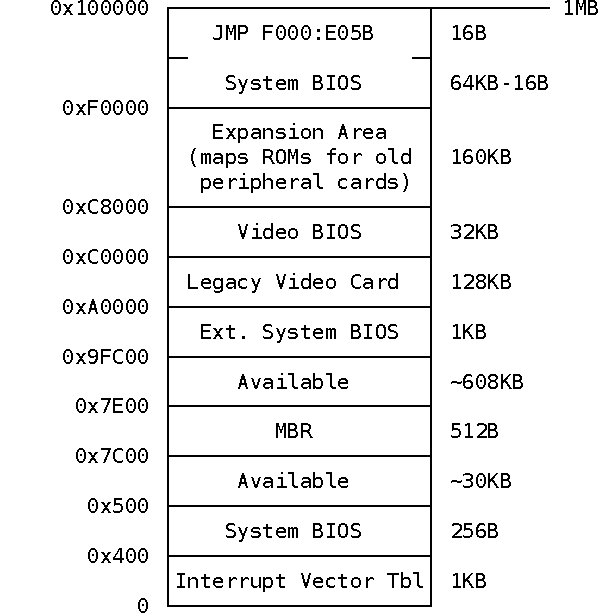
\includegraphics[width=.4\linewidth]{boot-mem}
  \caption{实模式下的内存布局}
  \label{fig:neicun}
\end{figure}

如图\ref{fig:neicun}所示,有两个可用的区
域\texttt{0x7E00~0x9FBFF}和\texttt{0x500~0x7BFF},本操作系统中将它放
在了\texttt{0x900}这个地方,所以最终MBR就会把Loader搬运到\texttt{0x900}这
个地方。

\section{内核的启动}
\label{sec:kernel}

\subsection{从实模式到保护模式}
\label{subsec:protect}

在Loader被搬运到\texttt{0x900}之后,需要将操作系统由实模式转变到保护模式\cite{LWY2013},原
因有以下几点:
\begin{itemize}
\item 实模式下操作系统和用户程序会属于同一个特权级。
\item 逻辑地址 = 物理地址,顾名思义就是用户程序引用的地址最终都指向真实的物理地址。
\item 用户程序能够自由地修改段基址。
\item 当需要访问超过64KB内存的区域时,要切换段基址。
\item 浪费计算机资源,因为一次只能够运行一个程序。
\item 一共只有20条地址线,加起来最大的可用内存也仅有1MB。
\end{itemize}

所以需要将操作系统引导到保护模式下才可以既安全,又能充分地利用计算机的
资源,还不用过于担心内存问题。

实模式的寻址方式是“(段基址:段内偏移
地址)”的形式;而保护模式的寻址方式是“(选择子:段:偏移地址)”,所以保护
模式还需要段描述符来描述一个段的信息,一个段描述符是8个字节,多个段描述
符就构成了段描述符表也就是“GDT”\footnote{GDT(Global Descriptor Table)\cite{chxs2012},全局描述符表,一个
  CPU对应一个GDT,它可以被放在内存的任何地方,也就是说它是全局的,存放在内存中的某个位置,
  而这个位置将由我们来指定}。因此第一步就是打开A20地址线(详见第\ref{sec:inprotect}节),让操作系
统能够访问更大的空间,方法也很简单,就是把\texttt{0x92}的第一个比特
置1就可以了。代码如下:
\begin{codeblock}
\begin{nasmcode}
in al, 0x92
or al, 0000_0010B
out 0x92, al
\end{nasmcode}  
\end{codeblock}
仅需要3行代码,就可以打开A20地址线。
之后加载之前写好的GDT。
最后一步就是将保护模式的开关 --- \texttt{CR0}寄存器 --- 的\texttt{PE}比特置1,也很简单,就三行代码:

\begin{codeblock}
\begin{nasmcode}
mov eax, cr0
or  eax, 0x00000001
mov cr0, eax
\end{nasmcode}  
\end{codeblock}

至此,操作系统已经成功进入了保护模式,接下来就是把CPU的使用权交给Kernel(内核)。

\subsection{内核初始化}

Loader会把内核从硬盘上读出来,然后加载到内存中去,至此,CPU的使用权就会传到内核手上
,这就是操作系统从电脑开机到接管CPU使用权的一个大致过程。内核的代码如下:

\begin{codeblock}
\begin{ccode}
int main(void)
{
    while(1);
}
\end{ccode}  
\end{codeblock}

没错,就可以是这么一个简单的程序,操作系统实质上从头到尾也就是在做这么一件
简单的事情。


%%% Local Variables:
%%% mode: latex
%%% TeX-master: "../thesis"
%%% End:
